\subsection{Precipitation-Runoff Modelling System (PRMS) (model ID: 45)}
The PRMS model (fig.~\ref{fig:45_schematic}) is a modelling system that, in its most recent version, allows the user to specify a wide variety of catchment processes and flux equations \citep{Markstrom2015}. The version presented here is a simplified version of the original PRMS model \citep{Leavesley1983}. Simplifications involve the use of PET time series instead of within-model estimates based on temperature, and simpler interception and snow routines. The model has 7 stores and 18 parameters ($TT$, $ddf$, $\alpha$, $\beta$, $STOR$, $RETIP$, $SCN$, $SCX$, $REMX$, $SMAX$, $c_{gw}$, $RESMAX$, $k_1$, $k_2$, $k_3$, $k_4$, $k_5$ and $k_6$). The model aims to represent:

\begin{itemizecompact}
\item Snow accumulation and melt;
\item Interception by vegetation;
\item Depression storage and impervious surface areas;
\item Direct runoff based on catchment saturation;
\item Infiltration into soil moisture and connection with deeper groundwater;
\item Potentially non-linear interflow, baseflow and groundwater sink.
\end{itemizecompact}

\subsubsection{File names}
\begin{tabular}{@{}ll}
Model: &m\_45\_prms\_18p\_7s \\
Parameter ranges: &m\_45\_prms\_18p\_7s\_parameter\_ ranges \\
\end{tabular}

% Equations
\subsubsection{Model equations}

% Model layout figure
{ 																	% This ensures it doesn't warp text further down
\begin{wrapfigure}{l}{6cm}
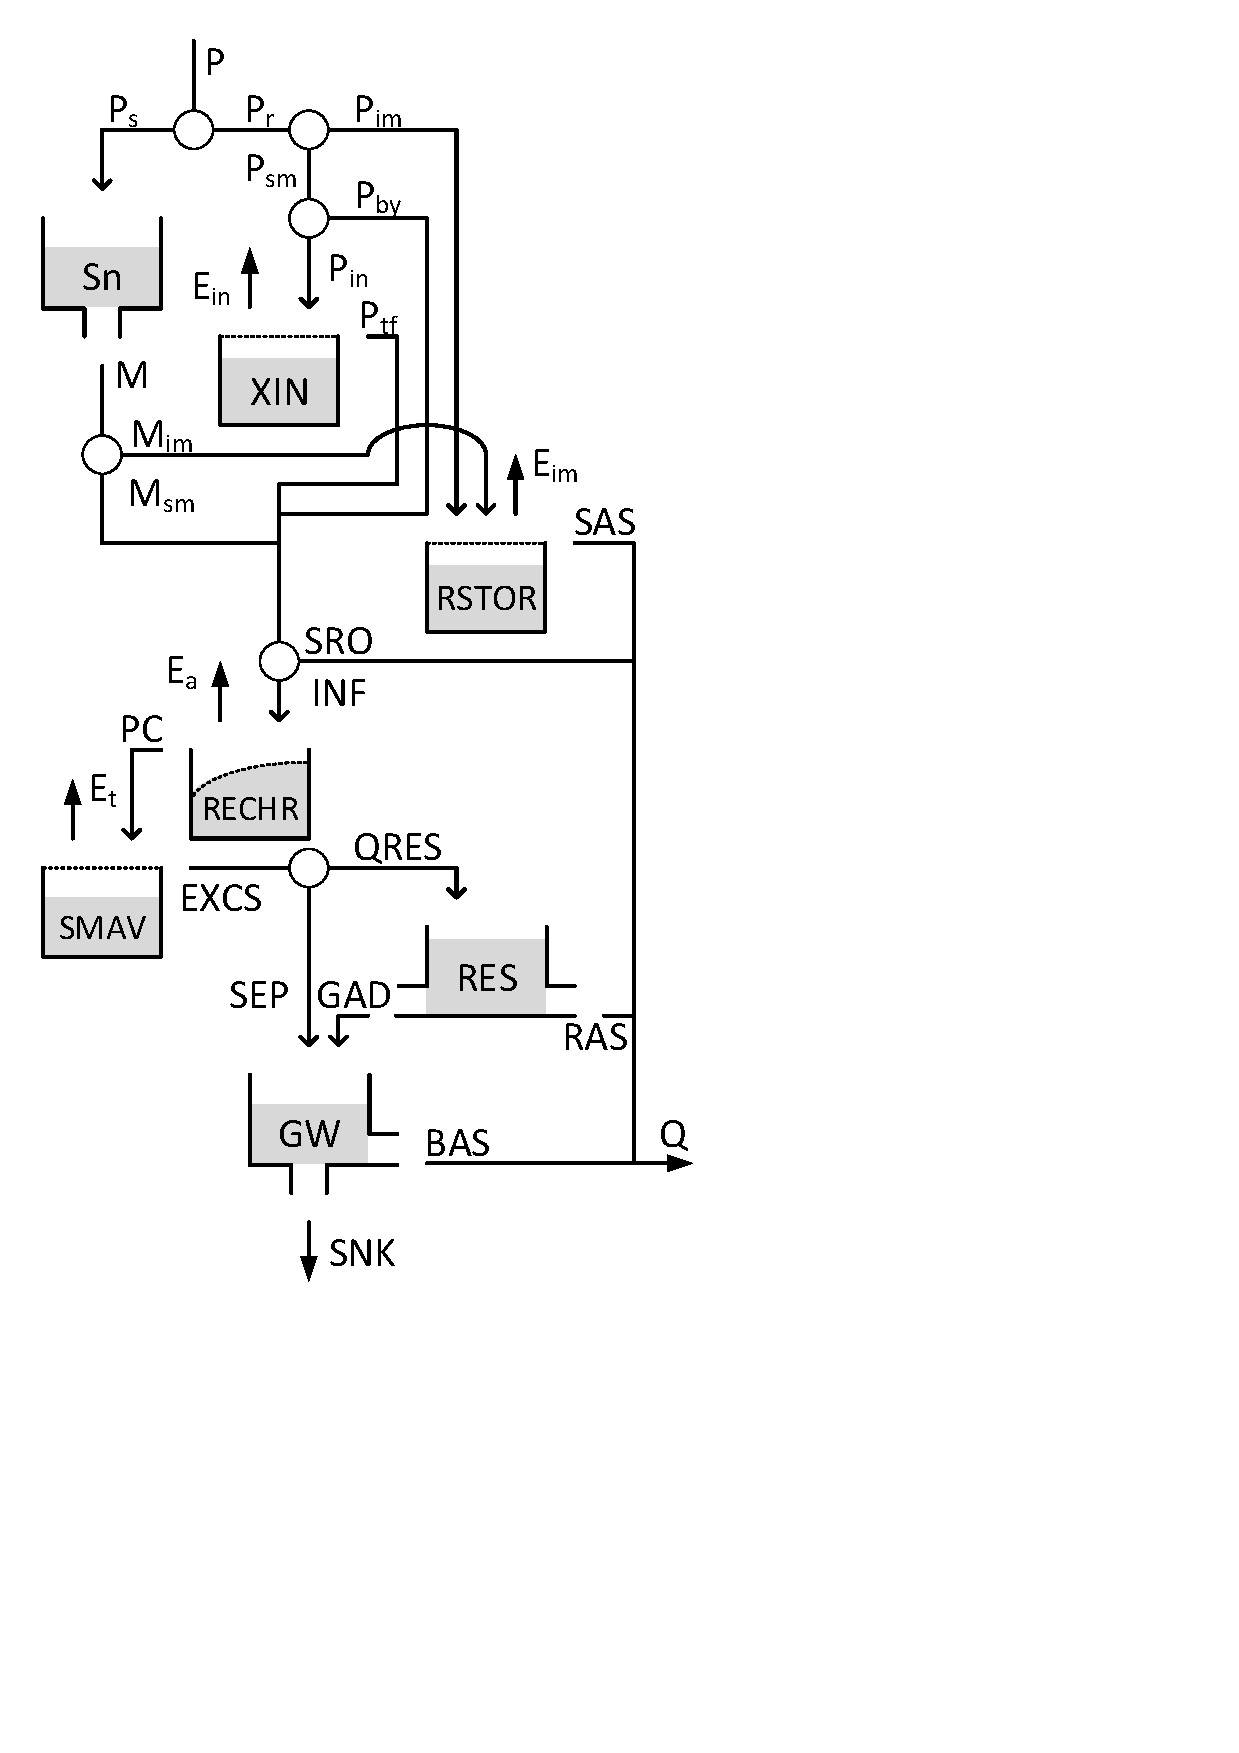
\includegraphics[trim=1cm 8cm 7cm 1cm,width=7cm,keepaspectratio]{./files/45_schematic.pdf}
\caption{Structure of the PRMS model} \label{fig:45_schematic}
\end{wrapfigure}

\begin{align}
	\frac{dSn}{dt} &= P_s-M \\
	P_s &= \begin{cases}
		P, &\text{if } T \leq TT \\
		0, & \text{otherwise} \\
	\end{cases} \\
	M &= 
	\begin{cases}
		ddf*(T - TT), & \text{if } T \geq TT \\
		0, & \text{otherwise}
	\end{cases}
\end{align}

Where S is the current snow storage [mm], $P_s$ the rain that falls as snow [mm], M the snowmelt [mm] based on a degree-day factor (ddf, [mm/\degree C/d]) and threshold temperature for snowfall and snowmelt (TT, [\degree C]).

} % end of wrapfigure fix

\begin{align}
	\frac{dXIN}{dt} &= P_{in} - E_{in} - P_{tf}\\
	P_{in} &= \alpha*P_{sm} \\
	P_{sm} &= \beta*P_r\\
	P_r &= \begin{cases}
		P, &\text{if } T > TT \\
		0, & \text{otherwise} \\
	\end{cases} \\
	E_{in} &= \begin{cases}
		\beta*E_p, & \text{if } XIN > 0 \\
		0, & \text{otherwise} \\
	\end{cases} \\
	P_{tf} &= \begin{cases}
		P_{in}, & \text{if } XIN = STOR \\
		0, & \text{otherwise}
	\end{cases}
\end{align}


Where $XIN$ [mm] is the current storage in the interception reservoir, recharged by intercepted rainfall $P_{in}$ $[mm/d]$ and drained by evaporation $E_i$ $[mm/d]$ and throughfall $P_{tf}$ $[mm/d]$. 
$P_{in}$ $[mm/d]$ is the fraction $\alpha$ [-] of rainfall on non-impervious area $P_{sm}$ $[mm/d]$ that does not bypass the interception reservoir. 
$P_{sm}$ $[mm/d]$ is the fraction $\beta$ [-] of rainfall $P_r$ $[mm/d]$ that does not fall on impervious area. 
Rainfall is given as all precipitation $P$ $[mm/d]$ that occurs when temperature $T$ [\degree C] is above a threshold $TT$ [\degree C]. 
$E_i$ $[mm/d]$ occurs at the potential rate $E_p$, corrected for the fraction of the catchment where interception can occur.
Throughfall $P_{tf}$ is all rainfall that reaches the interception reservoir when it is at maximum capacity $STOR$ [mm].

\begin{align}
	\frac{dRSTOR}{dt} &= P_{im} + M_{im} - E_{im} - SAS \\
	P_{im} &= (1-\beta)*P_r \\
	M_{im} &= (1-\beta)*M \\
	E_{im} &= \begin{cases}
		(1-\beta)*E_p, &\text{if } RSTOR > 0 \\
		0, &\text{otherwise} \\
	\end{cases} \\
	SAS &= \begin{cases}
		P_{im} +M_{im}, &\text{if } RSTOR = RETIP \\
		0, &\text{otherwise}
	\end{cases}
\end{align}

Where $RSTOR$ [mm] is current depression storage, refilled by rainfall and snowmelt on impervious area, $P_{im}$ $[mm/d]$ and $M_{im}$ $[mm/d]$ respectively, and drained by evaporation $E_{im}$  $[mm/d]$ and surface runoff $SAS$ $[mm/d]$. 
$P_{im}$ is given as the fraction $1-\beta$ of rainfall $P_r$. 
$M_{im}$ is given as the fraction $1-\beta$ of snowmelt $M$.
$E_{im}$ occurs at the potential rate $E_p$, corrected for the fraction of the catchment where impervious areas can occur.
$SAS$ occurs when the depression store is at maximum capacity $RETIP$ [mm].

\begin{align}
	\frac{dRECHR}{dt} &= INF - E_a - PC \\
	INF &= M_{sm} + P_{tf} + P_{by} - SRO\\
	M_{sm} &= \beta*M \\
	P_{by} &= (1-\alpha)*P_{sm}\\
	SRO &= \left[SCN+(SCX-SCN)*\frac{RECHR}{REMX}\right]*\left(M_{sm}+P_{tf} + P_{by}\right) \\
	E_a &= \frac{RECHR}{REMX}*\left(E_p-E_i-E_{im}\right)\\
	PC &= \begin{cases} 
		INF, &\text{if } RECHR = REMX \\
		0, &\text{otherwise}
	\end{cases}
\end{align}

Where $RECHR$ [mm] is the current storage in the upper soil moisture zone, recharged by infiltration $INF$ $[mm/d]$ and drained by evaporation $E_a$ $[mm/d]$ and percolation $PC$ $[mm/d]$.
$INF$ is the difference between incoming snowmelt $M_{sm}$ $[mm/d]$, throughfall $P_{tf}$ $[mm/d]$ and interception bypass $P_{by}$ $[mm/d]$, and surface runoff from saturated area $SRO$ $[mm/d]$. 
$S_{sm}$ is snowmelt from the fraction $\beta$ [-] of the catchment that is not impervious. 
$P_{by}$ is the fraction $1-\alpha$ of rainfall over non-impervious area $P_{sm}$ that bypasses the interception store.
$SRO$ has a linear relation between minimum contributing area $SCN$ [-] and maximum contributing area $SCX$ [-] based on current storage $RECHR$ and maximum storage $REMX$ [mm].
$E_a$ uses a similar linear relationship and accounts for already fulfilled evaporation demand by interception and impervious areas.
$PC$ occurs when the store reaches maximum capacity.

\begin{align}
	\frac{dSMAV}{dt} &= PC-E_t-EXCS\\
	E_t &=  \begin{cases} 
		\frac{SMAV}{SMAX}*\left(E_p-E_{in}-E_{im}-E_a\right), &\text{if } RECHR < \left(E_p-E_{in}-E_{im}\right)\\
		0, &\text{otherwise}\\
	\end{cases} \\
	EXCS &= \begin{cases} 
		PC, &\text{if } SMAV = SMAX-REMX \\
		0, &\text{otherwise}
	\end{cases}
\end{align}

Where $SMAV$ [mm] is the current storage in the lower soil moisture zone, recharged by percolation from the upper zone $PC$ $[mm/d]$ and drained by transpiration $E_t$ $[mm/d]$ and soil moisture excess $EXCS$ $[mm/d]$.
$E_t$ is corrected for already fulfilled evaporation demand and only occurs if the upper zone can not satisfy this demand. 
$E_t$ uses a linear relationship between current storage and the maximum storage in the lower zone $SMAX-REMX$ [mm].
$EXCS$ only occurs when the store has reached maximum capacity $SMAX-REMX$.

\begin{align}
	\frac{dRES}{dt} &= QRES-GAD-RAS\\
	QRES &= min(EXCS-SEP,0) \\
	GAD &= k_1\left(\frac{RES}{RESMAX}\right)^{k_2}\\
	RAS &= k_3*RES+k_4*RES^2\\
\end{align}

Where $RES$ [mm] is the current storage in the runoff reservoir, filled by the difference between soil moisture excess $EXCS$  $[mm/d]$ and constant groundwater recharge $SEP$  $[mm/d]$, and drained by groundwater drainage $GAD$  $[mm/d]$ and interflow component $RAS$  $[mm/d]$. 
$GAD$ is potentially non-linear using time coefficient $k_1$ $[d^{-1}]$ and non-linearity coefficient $k_2$ [-], and is also scaled by the maximum reservoir capacity $RESMAX$ [mm]. 
$RAS$ is non-linear interflow based on coefficients $k_3$ $[d^{-1}]$ and $k_4$ $[mm^{-1}d^{-1}]$.

\begin{align}
	\frac{dGW}{dt} &= SEP+GAD-BAS-SNK\\
	SEP &= min(c_{gw},EXCS) \\
	BAS &= k_5*GW\\
	SNK &= k_6*GW
\end{align}

Where $GW$ [mm] is the current groundwater storage, refilled by groundwater recharge from soil moisture $SEP$ and recharge from runoff reservoir $GAD$ and drained by baseflow $BAS$  $[mm/d]$ and flow to deeper groundwater $SNK$  $[mm/d]$.
$SEP$ occurs at the maximum rate $c_{gw}$ $[mm/d]$ if possible.
$BAS$ is a linear reservoir with time coefficient $k_5$  $[d^{-1}]$.
$SNK$ is a linear reservoir with time coefficient $k_6$ $[d^{-1}]$.
Total flow $Q_t$  $[mm/d]$:

\begin{align}
	Q_t &= SAS+SRO+RAS+BAS
\end{align}

\newpage
\subsubsection{Parameter overview}
% Table generated by Excel2LaTeX from sheet 'Sheet1'
\begin{table}[htbp]
  \centering
    \begin{tabular}{lll}
    \toprule
    Parameter & Unit  & Description \\
    \midrule
    $TT$  & $^oC$ & Threshold temperature for snowfall and snowmelt \\
    $ddf$ & $mm~^oC^{-1}~d^{-1}$ & Degree-day factor for snowmelt \\
    $\alpha$ & $-$   & Fraction of precipitation on soil that is intercepted \\
    $\beta$ & $-$   & Fraction of precipitation that falls on soil \\
    $STOR$ & $mm$  & Maximum interception storage \\
    $RETIP$ & $mm$  & Maximum depression storage \\
    $SCN$ & $-$   & Minimum contributing area to surface runoff \\
    $SCX$ & $-$   & Maximum contributing area to surface runoff \\
    $REMX$ & $mm$  & Maximum upper soil moisture storage \\
    $SMAX$ & $mm$  & Maximum total soil moisture storage \\
    $c_{gw}$ & $mm~d^{-1}$ & Maximum groundwater recharge rate \\
    $RESMAX$ & $mm$  & Maximum runoff routing storage \\
    $k_1$ & $d^{-1}$ & Runoff coefficient \\
    $k_2$ & $-$   & Runoff non-linearity \\
    $k_3$ & $d^{-1}$ & Runoff coefficient \\
    $k_4$ & $mm^{-1}~d^{-1}$ & Runoff coefficient \\
    $k_5$ & $d^{-1}$ & Runoff coefficient \\
    $k_6$ & $d^{-1}$ & Runoff coefficient \\
    \bottomrule
    \end{tabular}%
  \label{tab:addlabel}%
\end{table}%

